  \documentclass[14pt, oneside]{book}
    \usepackage[margin=1in]{geometry} 
    \usepackage[brazilian]{babel}
    \usepackage{graphicx}
    \usepackage[utf8]{inputenc}
    \usepackage[T1]{fontenc}
    \usepackage{amsmath,amsthm,amssymb,amsfonts, mathtools}
    \usepackage{enumitem, verbatim, tikz, multicol}
    \usepackage{titlesec,hyperref, color, float, comment}
    
        \hypersetup{
            colorlinks=false, %set true if you want colored links
            linktoc=all,     %set to all if you want both sections and subsections linked
            linkcolor=blue,  %choose some color if you want links to stand out
        }
    \usepackage{listings}
    \titleformat{\chapter}[hang]{\bf\huge}{\thechapter}{2pc}{}
    \DeclarePairedDelimiter{\ceil}{\lceil}{\rceil}
    \date{\vspace{-5ex}}
    \lstset{language=Python}  
    \usepackage{pythonhighlight}
     
    \newcommand{\N}{\mathbb{N}}
    \newcommand{\Z}{\mathbb{Z}}
    \newcommand\tab[1][1cm]{\hspace*{#1}}
    \renewcommand{\qedsymbol}{$\blacksquare$}
     
    
\theoremstyle{definition}
    \newtheorem{problem}{Problema}
    \newtheorem{dica}{Dica}
    \newtheorem{gabarito}{Gabarito}
    \newtheorem{defn}{Definição}
    \newtheorem{teorema}{Teorema}
    
\begin{document}
    \pagenumbering{gobble}

    \begin{titlepage}
        \centering 
        
\includegraphics[scale = 0.8]{ufpe.png} \\
        \Large{\textbf{UNIVERSIDADE FEDERAL DE PERNAMBUCO}}\\
        \large{Departamento de Eletrônica e Sistemas}
        \vspace*{\stretch{2.0}}
   
        \Huge\textbf{ELETRÔNICA DIGITAL}\\
        \Large\textbf{PORTA RETRATO MUSICAL}
   
        \vspace*{\stretch{2.0}}
        \vfill
        \Large{Arthur Santos Pimentel} \\
        \Large{Matheus Henrique Camilo de Araújo} \\
        \Large{Matheus Sobreira Farias} \\
        \Large{Pablo Godoy de Albuquerque}
        \\~\\
        \Large{Dezembro, 2018}
    \end{titlepage}

\addtocontents{toc}{\protect\hypertarget{toc}{}}
\tableofcontents
\mainmatter
        \chapter[Motivação]{\hyperlink{toc}{Motivação}}
            \tab Como explicado no projeto anterior, existem linguagens de descrição de Hardware que podem descrever o funcionamento de um circuito e, portanto facilitar o trabalho do projetista ao sintetizar seu projeto em forma de circuito. Neste projeto, com o auxílio da linguagem de descrição Verilog, pode-se observar o avanço devido às ferramentas disponibilizadas por uma linguagem. A grande economia de tempo acarreta na produtividade e agilidade da implementação de um projeto. Por exemplo, quando a linguagem de blocos no primeiro projeto foi usada, os grupos levaram em média duas semanas e meia para atingir as especificações do projeto. Agora, porém, com o auxílio de uma linguagem de descrição, nota-se a dificuldade criativa do projeto aumenta, enquanto a dificuldade da linguagem diminui, sendo esta a mais fácil de ser utilizada. \\
	        \tab Ainda pode-se dizer que o uso de uma linguagem possibilitou a discussão sobre certos pontos do projeto entre integrantes do grupo, já que a descrição dos circuitos se tornou um processo menos mecânico. Quando os integrantes do grupo se dividiam em tarefas, geralmente, as ideias surgiam e os circuitos eram manualmente implementados no \textit{Quartus}. Agora, porém, os circuitos são interpretados pelo programa através de uma linguagem em códigos e transformadas nas versões mais simplistas de seus circuitos. Assim, o grupo se preocupa menos com a estética e a legibilidade do bloco e passa a focar em suas funcionalidades.\\
	        \tab HDLs podem descrever o funcionamento do circuito, a sua concepção e organização, e ainda testá-lo para verificar seu funcionamento por meio de simulação. São padrões de expressões baseados em texto, da estrutura espacial, temporal e comportamental dos sistemas eletrônicos. Como outras linguagens de programação, HDLs incluem anotações explícitas para expressar a simultaneidade bem como sintaxe e semântica próprias. No entanto, em contraste com a maioria dos softwares de linguagem de programação, HDLs também incluem uma noção implícita de tempo, como um atributo primário de hardware. \\
	        \tab Verilog, cuja padronização atual é a IEEE 1364-2005, é uma linguagem de descrição de hardware (Hardware Description Language - HDL) usada para modelar sistemas eletrônicos ao nível de circuito. Essa ferramenta suporta o projeção, verificação e implementação de projetos analógicos, digitais e híbridos em vários níveis de abstração. Um dos principais atributos da modelagem de circuitos por linguagem descritiva frente à modelagem por captura de esquemático, é que desta maneira o projeto se torna independente da plataforma de desenvolvimento (IDE) na qual se está trabalhando. Além disso, adotando-se as boas práticas na descrição dos circuitos, o compilador é inclusive capaz de contornar a ausência de determinado recurso na tecnologia onde o circuito será sintetizado, conferindo uma portabilidade desse modelo para qualquer dispositivo (target) onde pode ser sintetizado. É uma linguagem chamada fortemente tipada. \\
	        \tab Geralmente, uma linguagem fortemente tipada tem regras de digitação mais rígidas em tempo de compilação, o que implica que erros e exceções são mais prováveis de acontecer durante a compilação. A maioria dessas regras afeta a atribuição de variáveis, os valores de retorno e a chamada de função. Essas linguagens são aquelas em que todas as variáveis tem um tipo específico e seus tipos são importantes para a linguagem. O que significa que uma vez que a variável foi declarada com um tipo ela será até o seu fim do mesmo tipo. Por outro lado, uma linguagem fracamente tipada possui regras de digitação mais flexíveis e pode produzir resultados imprevisíveis. %"ou pode executar conversão de tipo implícita em tempo de execução."
	        
           
            
        \chapter[Objetivos]{\hypertarget{obj}{}\hyperlink{toc}{Objetivos}}
             \tab Nesse projeto, foi utilizada a linguagem de descrição de Hardware Verilog, com o auxílio do software \textit{Quartus Prime 17.1} e da placa \textit{FPGA DE2-155}, ambos da \textit{Altera}, com o intuito de criar um porta retrato musical, seguindo os seguintes critérios:
            \begin{itemize}
                \item Existem três modos de operação. Estes são: Modo de Seleção, Modo de Exibição, Modo Vídeo.
                \item Chaves que compõem a placa devem ser usadas para selecionar as imagens no Modo de Seleção.
                \item Um botão é responsável por inicializar o porta retrato. Não é exibida nenhuma imagem ou som até este botão se apertado.
                \item Uma chave determina a ordem de exibição das imagens no Modo de Exibição e no Modo Vídeo.
                \item A música escolhida deve conter pelo menos cinco notas musicais.
                \item Dois botões devem ser usados para controlar o volume da música.
            \end{itemize}
            
            
        \chapter[Desenvolvimento]{\hyperlink{toc}{Desenvolvimento}}
            \tab Para realizar a implementação do jogo de repetição, foi utilizado o software \textit{Quartus Prime 17.1}, que é um software cuja função é ser um ambiente de desenvolvimento para linguagens de descrição de hardware, sendo assim, a placa a qual foi descrita pelo projeto foi a \textit{Altera DE2-115}. Foi utilizada ao longo do desenvolvimento a linguagem de descrição de hardware Verilog. \\
    
            
            \section[O VGA]{\hyperlink{toc}{O VGA}}
            \tab O VGA é uma interface padrão para controlar a imagem gerada num monitor analógico. Essa interface depende de sinais como os de sincronização vertical e horizontal, além dos sinais responsáveis por fornecer as cores dos pixels.
            
            
            \tab Os sinais de sincronização são pulsos digitais que sincronizam os demais sinais com o monitor. Já os sinais de cores são sinais analógicos, que variam de 0 a 0.7V, e são responsáveis pelas intensidades de cada uma das cores responsáveis pela formação de um pixel: vermelho, verde e azul.
            
             \tab Existe uma grande variedade de modos para o padrão VGA, cada um com uma resolução e uma taxa de atualização específica. Cada um desses modos possui parâmetros de tempo bem definidos. Utilizar os parâmetros certos, para o modo que se deseja, é extremamente crucial para a obtenção de um resultado correto. O controlador VGA necessita que o usuário forneça um pixel clock. Na FPGA, ele pode ser obtido utilizando um PLL (phase-locked loop). Para uma resolução de 640x480, a uma taxa de atualização de 60Hz, por exemplo, esse pixel clock deve ser de 25.175MHz.
             
              \begin{figure}[H]
                    \centering
                    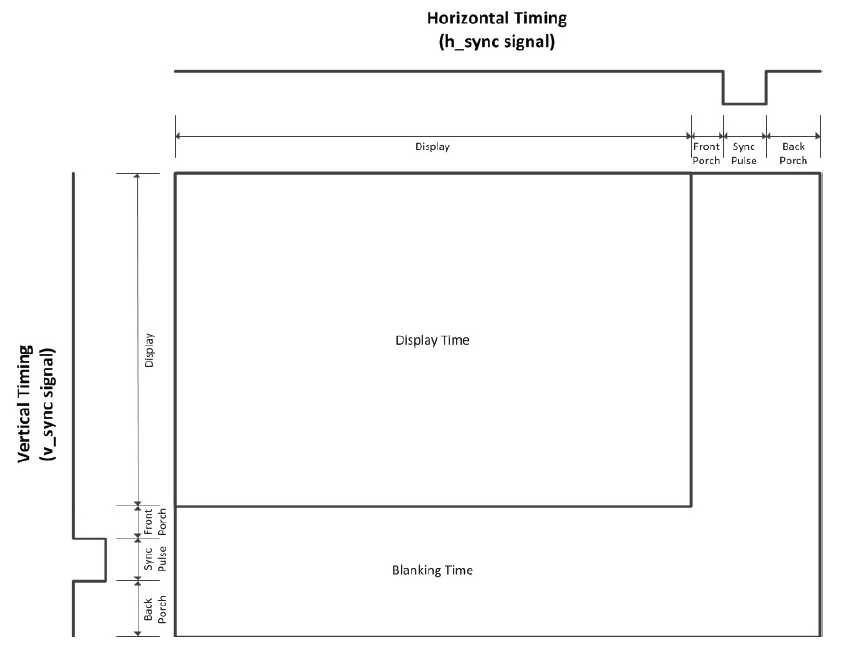
\includegraphics[scale=0.8]{vga.PNG}
                    \caption{Esquemática tida como referência para elaboração do projeto.}
                    \label{vga}
                \end{figure}
             
             \tab A figura \ref{vga} mostra os sinais de tempo produzidos pelo controlador de VGA utilizado
no projeto. Esse controlador possui dois contadores, o primeiro incrementa com o pixel
clock e controla o tempo do sinal h\_sync. Fazendo esse contador começar do zero, temos,
com ele, o controle do número da coluna em que se está, atualmente. O tempo de exibição
horizontal é seguido por um tempo em branco, necessário para o funcionamento devido
do equipamento.
O outro contador é incrementado sempre que se completa uma linha e, portanto,
quando setado para começar do zero, indica justamente a linha da tela onde o programa
se encontra. Como antes, essa exibição vertical também é seguida por um tempo em
branco. Quando esse tempo termina, o contador reseta e é iniciada a atualização para a
nova tela a ser impressa.
Dessa forma, utilizando estes contadores, o controlador emite como saída os sinais de
sincronização horizontal e vertical, assim como o enable do display (que é um AND lógico
entre os tempos horizontal e vertical), e as coordenadas de linha e de coluna do pixel.
             
             
             
             
            
            \section[A Memória Flash]{\hyperlink{toc}{A Memória Flash}}
            
               \tab  A memória flash é uma memória do tipo EEPROM (Electrically-Erasable Programmable Read-Only Memory), cujos chips são semelhantes aos da Memória RAM, que permite que diversos endereços sejam apagados ou escritos numa só operação. Dessa forma, é um chip regravável, ao contrário da memória RAM convencional.
               
               \tab A placa DE2-115 contem uma memória flash de 8MB com barramento de dados de 8 bits. Observa-se na Figura \ref{conexões flash} as conexões entre o FPGA e a Flash.
               
                \begin{figure}[H]
                    \centering
                    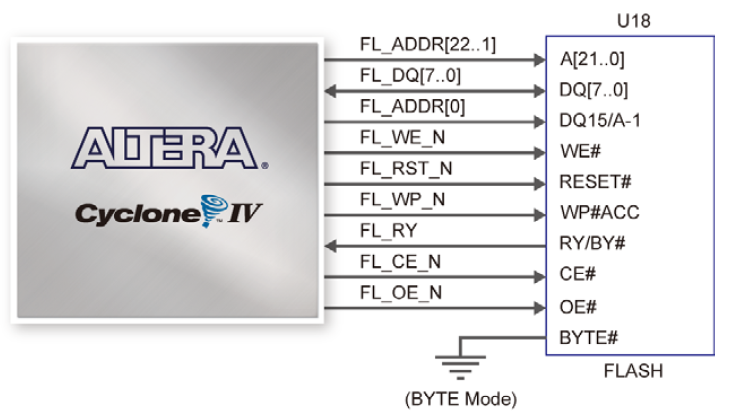
\includegraphics[scale=0.8]{flash.PNG}
                    \caption{Conexões entre FPGA e Memória Flash.}
                    \label{conexões flash}
                \end{figure}
                    
                
            \section[Conversão de Imagens e  Escrita na Flash]{\hyperlink{toc}{Conversão de Imagens e  Escrita na Flash}}
            
                \tab Antes de gravar as imagens escolhidas na memória Flash, necessita-se primeiro converte-las para um formato adequado. Assim, com o auxílio do software \textit{Microsoft Paint}, converte-se as imagens selecionadas para o formato Bitmap de 256 cores (*.bmp). Em seguida, com o auxílio do software \textit{MATLAB}, converte-se as imagens para o formato *.hex, seguido do mapa de cores das imagens.
                
                \tab Finalmente, o processo de escrita na memória flash se dá pelo \textit{Control Panel}, apaga-se o conteúdo presente na Flash e grava-se o mapa de cores seguido pelas imagens convertidas, lembrando de seleciona o endereço de escrita dos arquivos. 
                
                \tab Observa-se na Figura \ref{control panel} o Painel de Controle em que é feito a escrita na memória Flash.
                    
                     \begin{figure}[H]
                    \centering
                    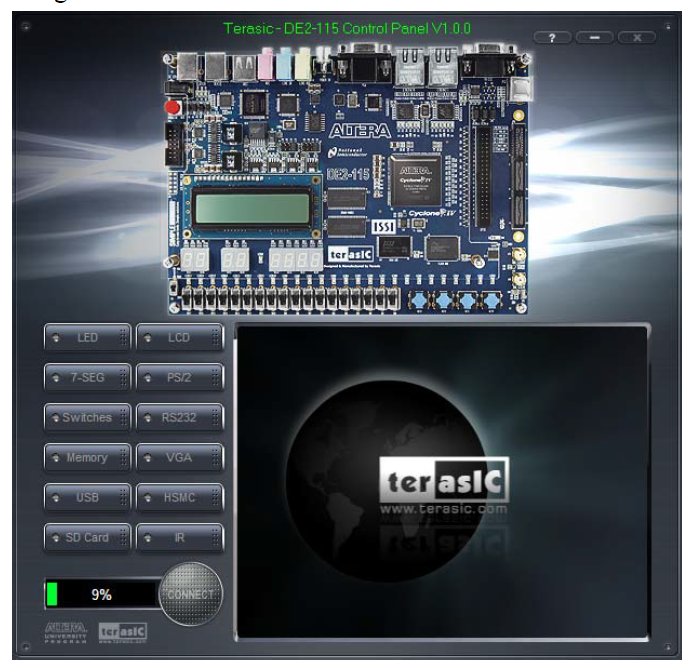
\includegraphics[scale=0.7]{control_panel.PNG}
                    \caption{Painel de Controle da FPGA.}
                    \label{control panel}
                \end{figure}
                
            \section[Leitura da Flash]{\hyperlink{toc}{Leitura da Flash}}
                
                \tab Implementou-se um código em Verilog apra realizar a leitura dos dados da Flash. Esse código foi acrescentado ao código padrão da placa, DE2\_115\_Default.v. Um dos precedimentos consiste em selecionar o endereço da Flash a ser lido. Implementou-se essa lógica por meio de uma declaração CASE que associa o endereço a ser lido à uma variável "select". Esta variável, por sua vez, pode ser associada às chaves presentes na placa ou à um contador, dependendo do modo de operação de exibição das imagens.
                
                \tab Observa-se a implementação dessa lógica na Figura \ref{leitura endereço}.
                    
                    \begin{figure}[H]
                    \centering
                    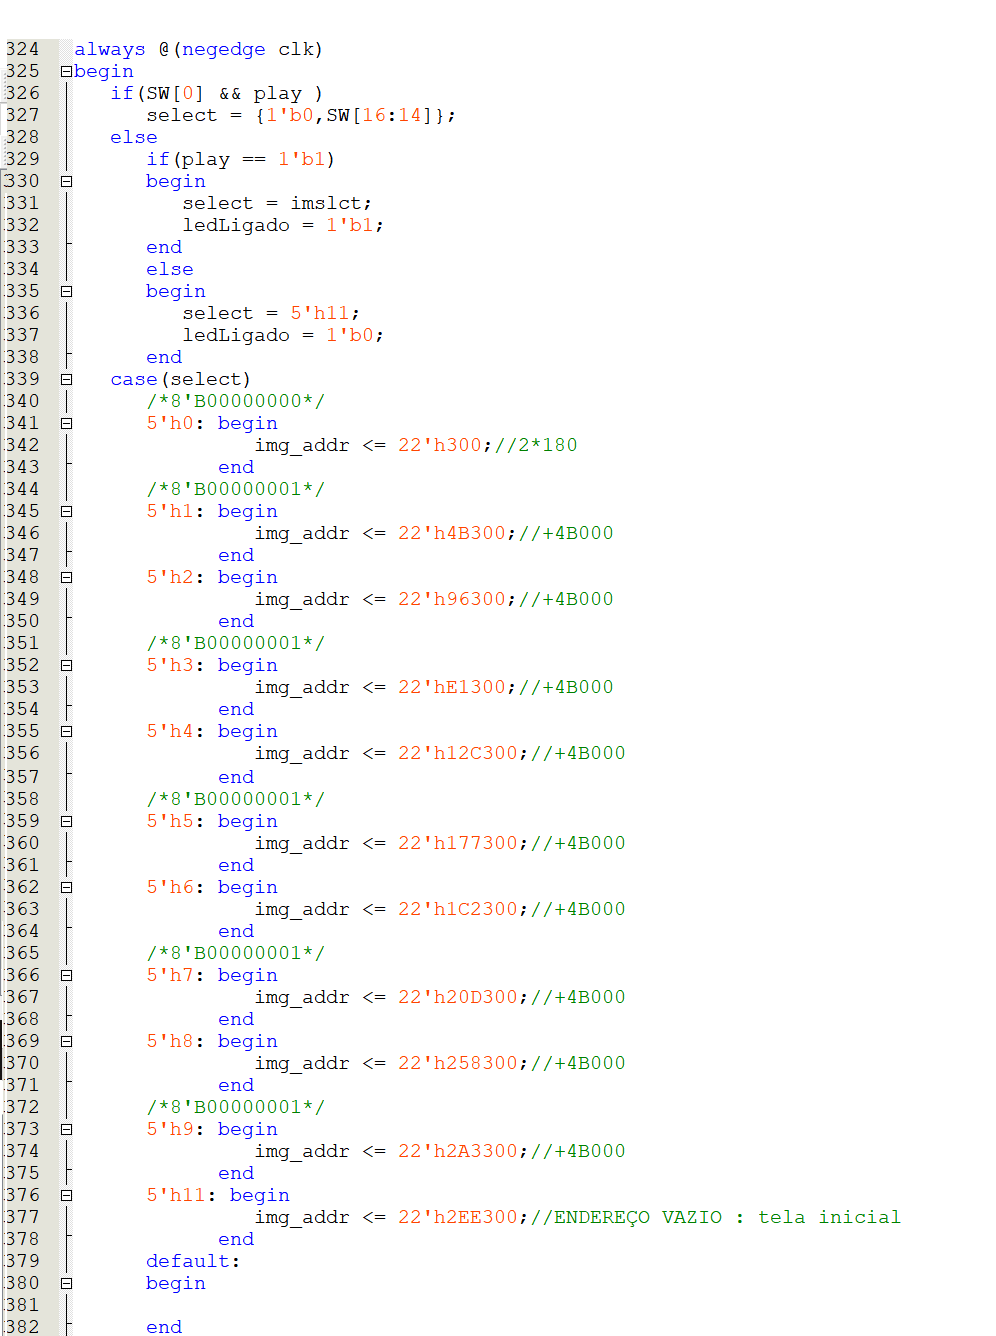
\includegraphics[scale=0.7]{leitura_endereco.png}
                    \caption{Código em Verilog para Seleção de Endereço de leitura da Flash.}
                    \label{leitura endereço}
                \end{figure}
                
            \tab Além disso, necessitou-se implementar uma lógica para o caso dos modos de operação de Seleção e de Vídeo. Em que, utiliza-se três variáveis para controlar o modo de operação, o tempo de exibição das imagens e a ordem de exibição. 
            
            \tab Nesta lógica, usa-se a variável SW[1] para determinar tempo de exibição das imagens, e consequentemente, o modo de operação (5 segundos para o Modo de Exibição e 0,2 segundos para o Modo Vídeo). Ademais, a variável "crescente" determina se a ordem de exibição, sendo acrescido ou decrescido o valor da variável "imslct", que funciona como um contador.
            
            \tab A lógica desse código pode ser vista na Figura \ref{logica modo}.
            
                \begin{figure}[H]
                    \centering
                    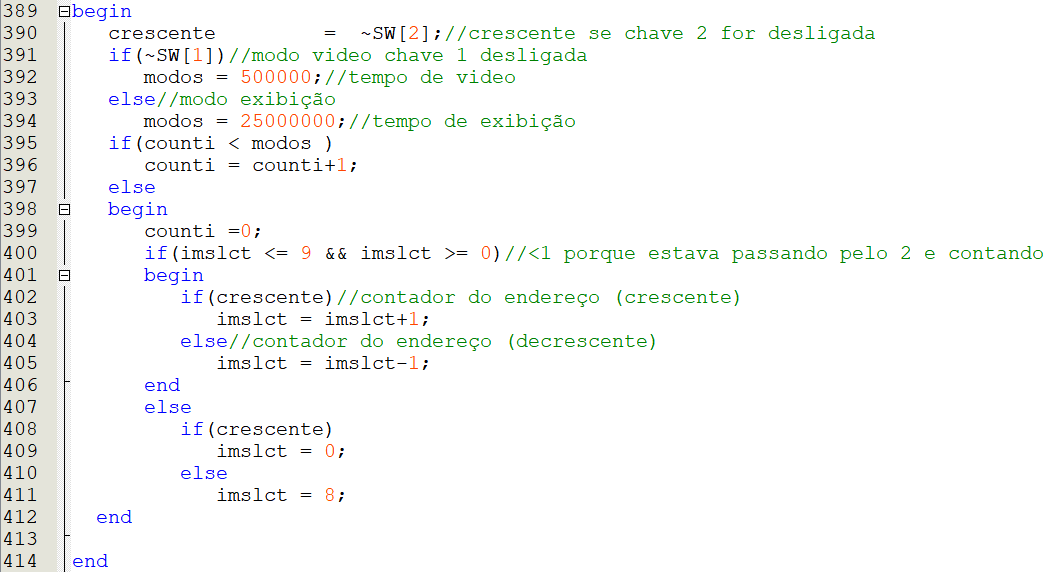
\includegraphics[scale=0.7]{logica_modo.PNG}
                    \caption{Código em Verilog para Controlar Modo de Operação, Tempo e Ordem de Exibição das Imagens.}
                    \label{logica modo}
                \end{figure}
            
            \section[CODEC de Áudio]{\hyperlink{toc}{CODEC de Áudio}}
                O CODEC de áudio nada mais é que um codificador/decodificador elaborado para controlar as funções de áudio da placa DE2-115. Este módulo foi separado em 3 ambientes, como mostrado na Figura \ref{fig:codec}
                
                \begin{figure}[!h]
                        \centering
                        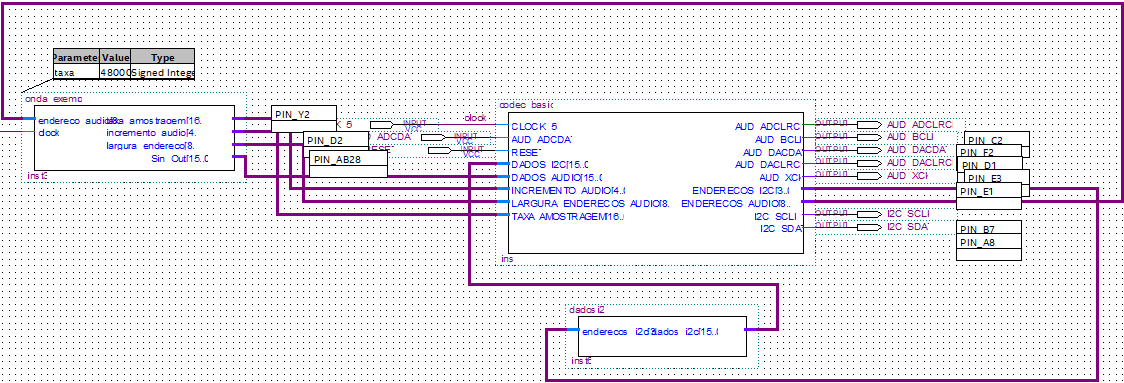
\includegraphics[scale=0.7]{codec.png}
                        \caption{CODEC}
                        \label{fig:codec}
                    \end{figure}
                
                \subsection[codec basico]{\hyperlink{toc}{codec basico}}
                    Tal ambiente tem como funcionalidade tratar os dados recebidos pelos outros ambientes, de tal forma a endereçar saídas e entradas corretamente, o bloco e seu código de configurações é mostrado na Figura \ref{fig:codecbasico}
                    
                    \begin{figure}[!h]
                        \centering
                        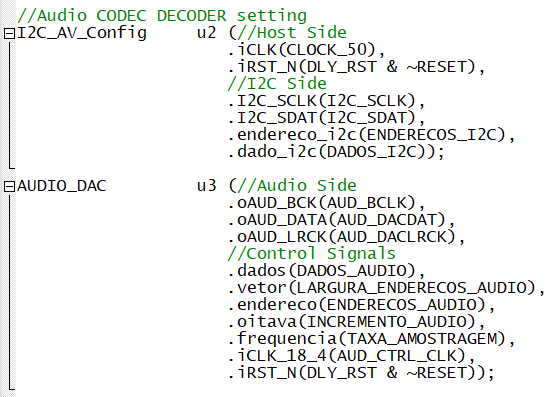
\includegraphics[scale=1]{config.png}
                        \caption{codec basico}
                        \label{fig:codecbasico}
                    \end{figure}
                
                \subsection[dadosi2c]{\hyperlink{toc}{dadosi2c}}
                    Tal ambiente tem como funcionalidade enviar os dados protocolados segundo o protocolo i2c, esses dados são armazenados em um vetor de endereços onde a cada endereço é atribuido uma função diferente, sendo volume, definição de CLOCK, ativação de carga simultânea, definição de taxa de amostragem, etc.
                    
                    \begin{figure}[!h]
                        \centering
                        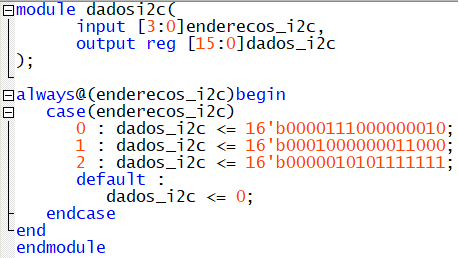
\includegraphics[scale=1]{dadosi2c.png}
                        \caption{dadosi2c}
                        \label{fig:dadosi2c}
                    \end{figure}
                    
                \subsection[onda exemplo]{\hyperlink{toc}{onda exemplo}}
                    Tal ambiente se foi necessário, pois, um dos objetivos do projeto era utilizar o CODEC para tocar alguma música enquanto o vídeo era mostrado na tela. Pela decisão unânime do grupo, a música escolhida foi o tema do anime Naruto, chamada Sadness and Sorrow, adaptada de forma que fosse melhor audível, primeiramente, necessitou-se identificar cada nota correspondente à música e seu tempo de duração, algo que não foi difícil pois integrantes da equipe possuem conhecimento teórico de música. Posteriormente, para cada nota identificada, necessitou-se encontrar a frequência correspondente, algo que também não foi difícil pois a tabela de frequências correspondentes a cada nota é facilmente encontrada na internet, sendo a tabela utilizada exposta na Figura \ref{fig:tabela} e as notas de Sadness and Sorrow na ordem, expostas na Figura \ref{fig:notas}.
                    \begin{figure}[!h]
                        \centering
                        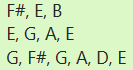
\includegraphics[scale=1]{notas.png}
                        \caption{Notas da Música Sadness and Sorrow}
                        \label{fig:notas}
                    \end{figure}
                    \begin{figure}[!h]
                        \centering
                        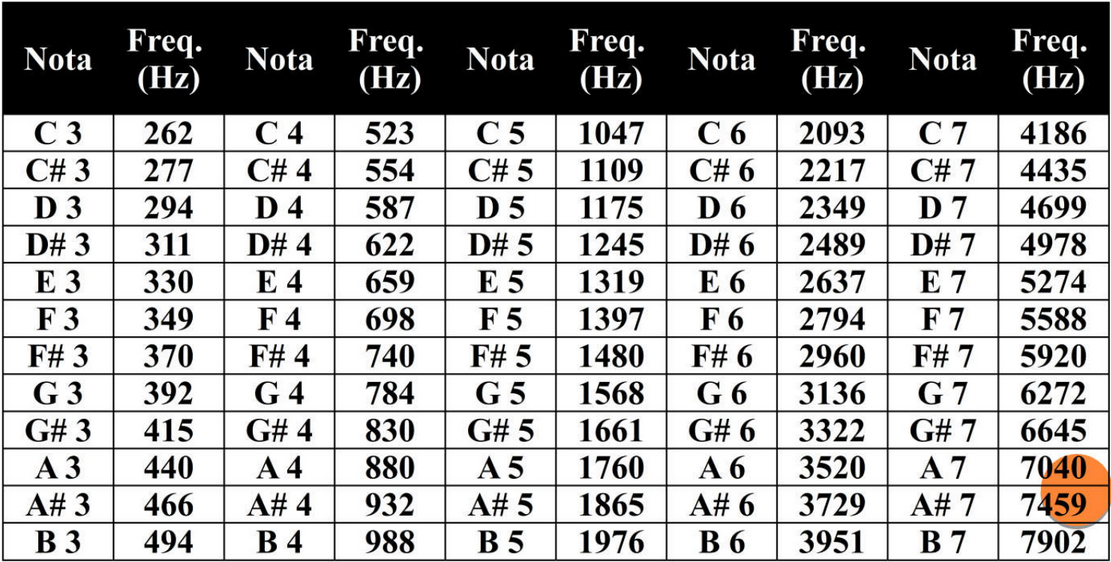
\includegraphics[scale=0.7]{tabela.png}
                        \caption{Tabela de Notas e suas Frequências Correspondentes}
                        \label{fig:tabela}
                    \end{figure}
                    Uma vez sabendo as frequências correspondentes a cada nota, necessitou-se, agora, definir uma taxa de amostragem para a função contínua que representa o sinal emitido pela onda correspondente a tal frequência, para então discretizar a onda, sendo possível ser trabalhada no software Quartus. Foi definido uma taxa de amostragem de $48000$, valor arbitrário, não precisava ser tão grande visto que as notas determinadas não possuem uma frequência muito alta. Sendo assim, foi elaborado um código em Python que, dado uma função senoide de uma frequência fornecida, e também com uma taxa de amostragem definida, o código retorna uma tabela que caracteriza a nota do formato usado no código em Verilog, mostrado na Figura \ref{fig:python}
                    
                    \begin{figure}[!h]
                        \centering
                        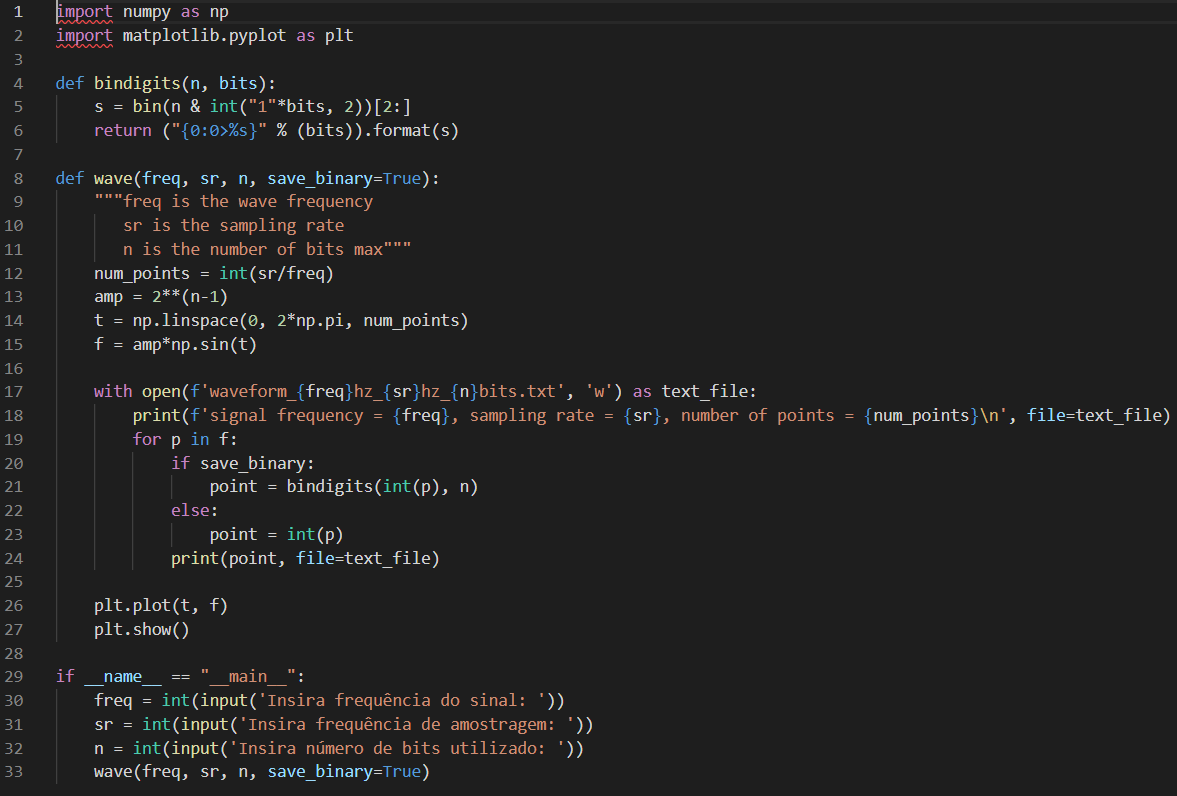
\includegraphics[scale=0.7]{python.png}
                        \caption{Código em Python}
                        \label{fig:python}
                    \end{figure}
                    
                    Tendo a tabela montada dos pontos de cada nota, como por exemplo a nota A ($440$ Hz), mostrado na Figura \ref{fig:a} foi criado uma maquina de estados para determinar o tempo que cada nota é tocada, mostrado na Figura \ref{fig:maquina}.
                    
                    \begin{figure}[!h]
                        \centering
                        
\includegraphics[scale=0.7]{a.png}
                        \caption{Nota A ($440$ Hz)}
                        \label{fig:a}
                    \end{figure}
                    
                    \begin{figure}[!h]
                        \centering
                        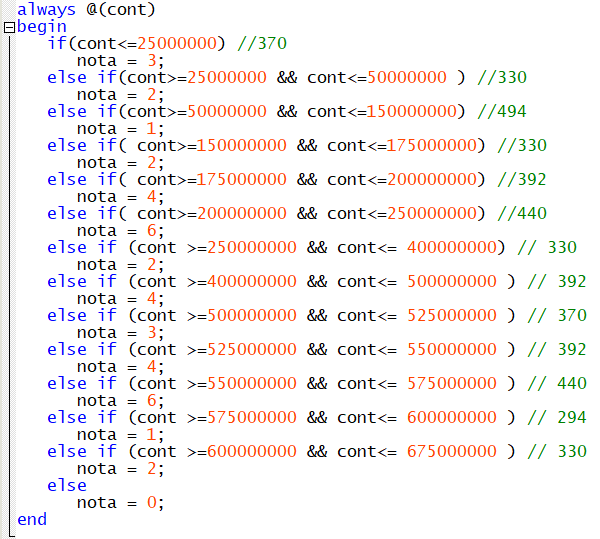
\includegraphics[scale=0.7]{maquina.png}
                        \caption{Maquina de Estados}
                        \label{fig:maquina}
                    \end{figure}
                
                
         \chapter[Manual de Operação]{\hyperlink{toc}{Manual de Operação}}
                \tab Esta seção é dedicada a esclarecer o funcionamento e organização da placa da \textit{Altera DE2-115}, bem como explicitar quais chaves, displays, LEDs e botões foram utilizados na implementação do jogo de repetição. \\
                \tab Observa-se um esquemático da placa na Figura \ref{manual}. Em que:
              
                \begin{itemize}
                    \item SW[0] e SW[1] em conjunto determinam o modo de operação das imagens. SW[0] também determina a função \textit{mute} do código do som. 
                    \item SW[2] determina se a exibição das imagens será crescente ou decrescente nos modos exibição e vídeo.
                    \item SW[17] a SW[14] selecionam as imagens no modo de Seleção.
                    \item O primeiro push-button inicializa a exibição da primeira imagem após o acionamento da placa. 
                \end{itemize}
                
                \begin{figure}[H]
                    \centering
                    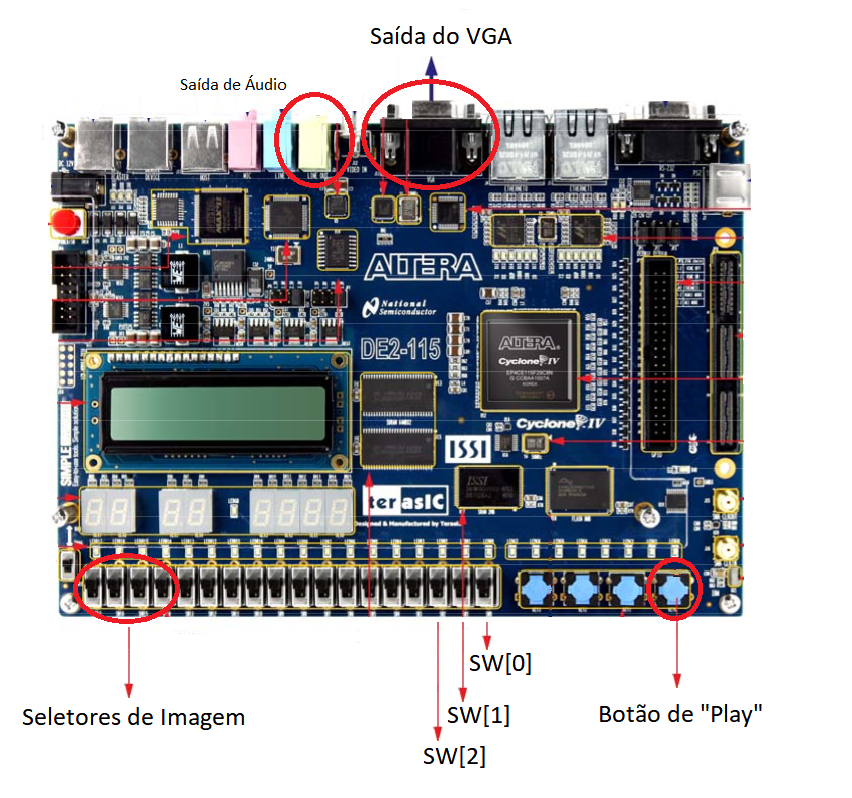
\includegraphics[scale=0.9]{manual.png}
                    \caption{Manual de Operação.}
                    \label{manual}
                \end{figure}\\
                
                
         
         \chapter[Resultados]{\hyperlink{toc}{Resultados}}
            
            \tab Observa-se a seguir, as imagens salvas na memória Flash da Placa que serão exibidas na tela do computador por meio do VGA. 
            
                \begin{multicols}{2}
                    \begin{figure}[H]
                        \centering
                        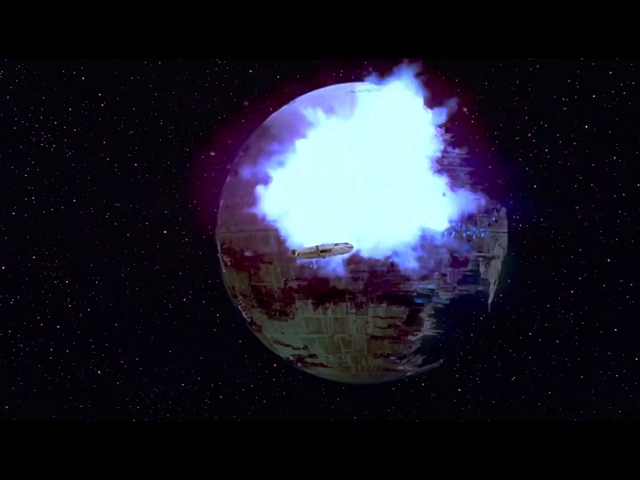
\includegraphics[scale=0.65]{img1.png}
                        \caption{Imagem 1.}
                        \label{manual}
                     \end{figure}
                
                    \begin{figure}[H]
                        \centering
                        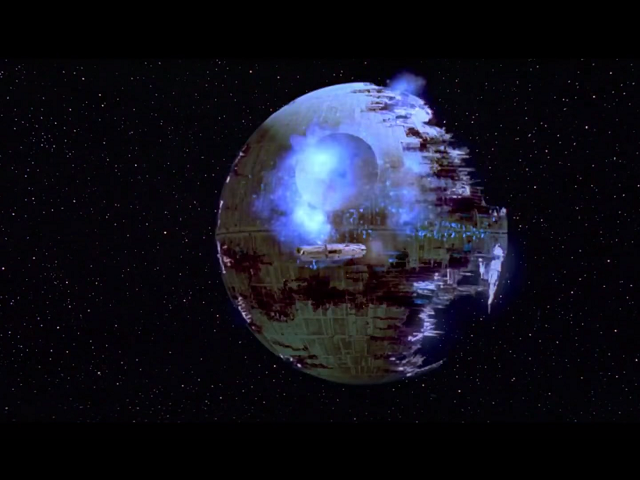
\includegraphics[scale=0.65]{img2.png}
                        \caption{Imagem 2.}
                        \label{manual}
                    \end{figure}
              
                     \begin{figure}[H]
                        \centering
                        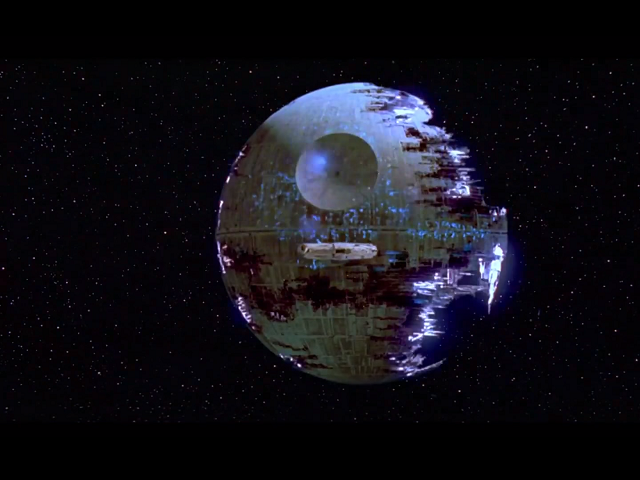
\includegraphics[scale=0.65]{img3.png}
                        \caption{Imagem 3.}
                        \label{manual}
                     \end{figure}
                
                    \begin{figure}[H]
                        \centering
                        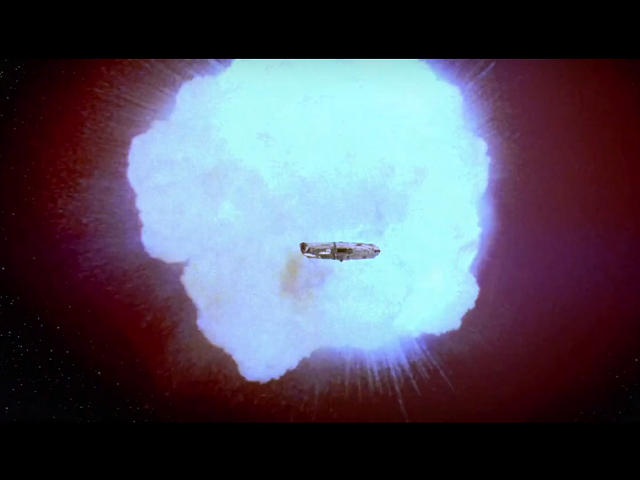
\includegraphics[scale=0.65]{img4.png}
                        \caption{Imagem 4.}
                        \label{manual}
                    \end{figure}
                    
                     \begin{figure}[H]
                        \centering
                        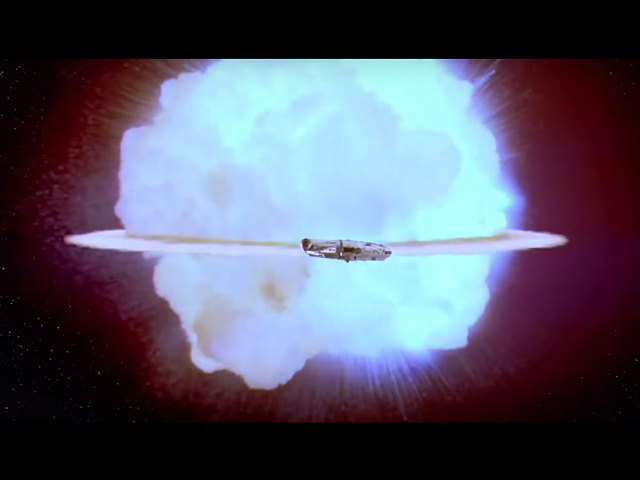
\includegraphics[scale=0.65]{img5.png}
                        \caption{Imagem 5.}
                        \label{manual}
                     \end{figure}
                
                    \begin{figure}[H]
                        \centering
                        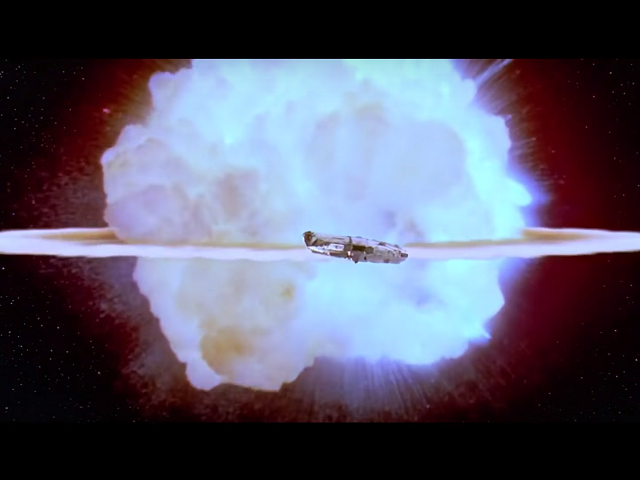
\includegraphics[scale=0.65]{img6.png}
                        \caption{Imagem 6.}
                        \label{manual}
                    \end{figure}
                
                     \begin{figure}[H]
                        \centering
                        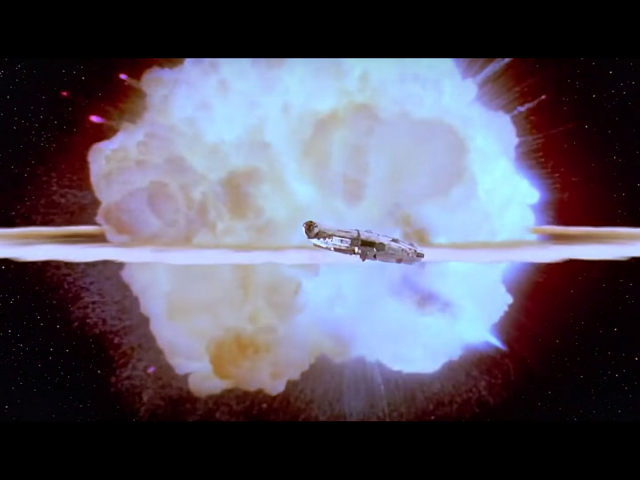
\includegraphics[scale=0.65]{img7.png}
                        \caption{Imagem 7.}
                        \label{manual}
                     \end{figure}
                
                    \begin{figure}[H]
                        \centering
                        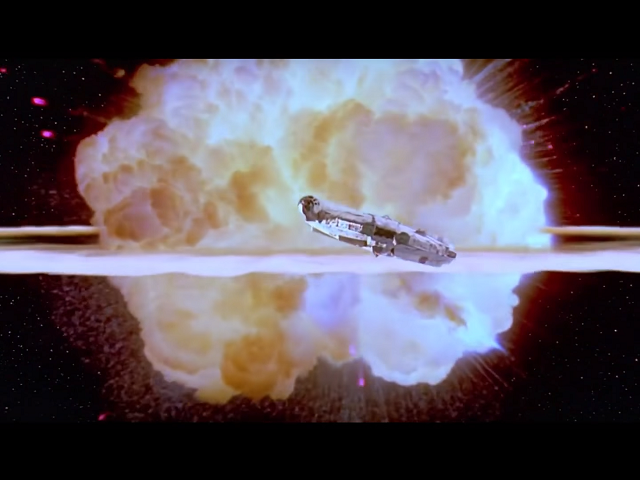
\includegraphics[scale=0.65]{img8.png}
                        \caption{Imagem 8.}
                        \label{manual}
                    \end{figure}
                    
                     \begin{figure}[H]
                        \centering
                        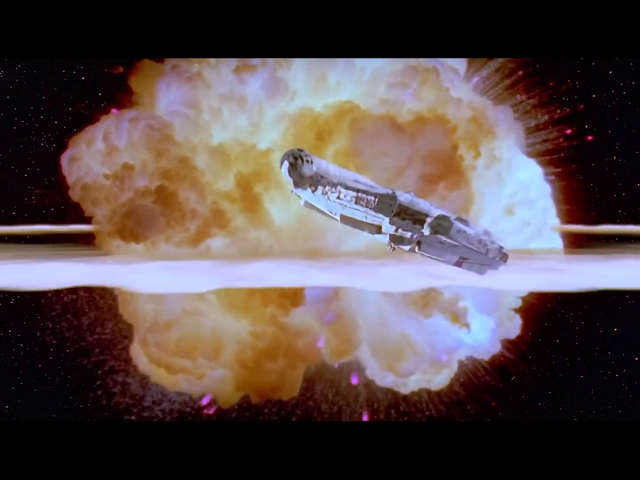
\includegraphics[scale=0.65]{img9.png}
                        \caption{Imagem 9.}
                        \label{manual}
                     \end{figure}
                
                    \begin{figure}[H]
                        \centering
                        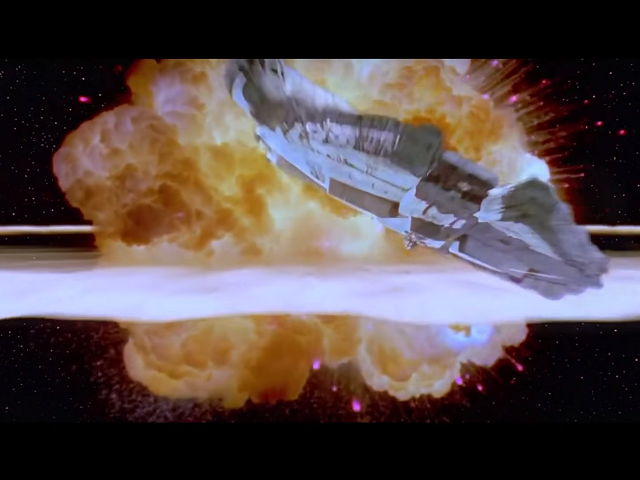
\includegraphics[scale=0.65]{img10.png}
                        \caption{Imagem 10.}
                        \label{manual}
                    \end{figure}
                
                
                \end{multicols}
               
            
        \chapter[Discussão]{\hyperlink{toc}{Discussão}} \hypertarget{ana}{}
            \tab Neste projeto, diferentemente dos outros, alguns problemas ocorreram e impediram a conclusão da programação das funcionalidades desejadas desde o princípio. A começar pela leitura da memória flash. Ao observar o funcionamento do módulo VGA, nota-se que as imagens estão sendo propriamente lidas da memória flash da placa, assim como planejado. Porém, infelizmente, o grupo enfrentou algumas adversidades, como a falta de tempo, ao longo dessas últimas duas semanas e acabou por escolher, estrategicamente, implementar o módulo de áudio separadamente. Desta forma, o circuito descrito por este grupo, quanto ao áudio, performa normalmente, porém, não lê as informações diretamente da memória flash. Pelo contrário, escolheu-se implementar a música nota por nota, na devida sequência, e usar contadores para determinar o tempo para cada nota. 
            
         
          %  Notou-se, claramente, que as tarefas exigidas eram, de certa forma, de dificuldade mediana. Entretanto, o período 2018.2 provou ser atípico, culminando muito tarde e de maneira turbulenta para a maior parcela de alunos que estão matriculados nesta disciplina. Portanto, não é difícil imaginar que, assim como este grupo, outros também enfrentaram a falta de tempo e, logo, entregarão um projeto inacabado, como este. Uma observação segue: por diversas vezes este grupo, e outros também, encontrou o laboratório fechado no horário de funcionamento. Por vezes, o laboratório era aberto bem após o horário previsto e fechado bem antes do encerramento oficial das atividades do dia. Esta prática recorrente, apesar de não ser gravíssima, atrapalhou o andamento dos projetos de vários grupos, de modo que, se questionados, outros discentes confirmarão esta observação.
         
            
            \tab É importante explicar outra particularidade deste projeto. Quando as partes implementadas separadamente foram incorporadas, o grupo enfrentou várias dificuldades com a interface de conexão das mesmas e, novamente, pela falta de tempo, este foi outro problema sem solução. Optou-se, assim, por apresentar os códigos funcionando separadamente, isto é, o CODEC de áudio e o VGA não estão sob uma mesma hierarquia. 
                
        \chapter[Conclusão]{\hyperlink{toc}{Conclusão}}
            \tab Conclui-se aqui o último projeto da disciplina de Eletrônica Digital. Ao longo deste período três linguagens de descrição de Hardware foram experimentadas e cada uma delas ofereceu benefícios únicos. Verilog, em contraste com as outras linguagens, ofereceu certas facilidades, das quais destaca-se a proximidade com uma linguagem de programação orientada a objetos, como C. Com isso, certos comandos se tornam bastante intuitivos e de fácil interpretação. Além disso, a descrição de circuitos mais complexos se torna mais enxuta, às vezes. Portanto, nota-se a riqueza desta linguagem e, desta forma, sua importância para a formação do profissional é, assim, reafirmada.
            
             Quanto aos resultados obtidos, considerou-se que, apesar dos problemas já identificados previamente, o projeto encontra-se devidamente apresentável e praticável. A música selecionada está sendo reproduzida e as imagens selecionadas estão sendo exibidas em sequência e em forma de vídeo, dependendo do comando. Apesar da memória determinada não ter sido trabalhada para informar as amplitudes das senoides, o módulo VGA opera a flash de maneira satisfatória. Logo, o grupo considera o projeto um sucesso, mesmo que parcial. 
                    

\end{document}